\section{Malus's law}

    \subsection{Theory of Malus's law}
    Malus's law describes the intensity of polarized light after passing through a polarizer, it's derivation can be found in the appendix
    \ref{sec:derivationmalus}. It states that the intensity $I$ of the transmitted light is
    related to the intensity $I_0$ of the incident light and the angle $\theta$ between the light's initial polarization direction and the axis of the polarizer
    by the equation:
    \begin{equation}
        I = I_0 \cos^2(\theta)
        \label{eq:Malus}
    \end{equation} 
    After passing through the polarizer, the light is polarized along the axis of the polarizer. The wave components that are not transmitted are absorbed
    by the polarizer, resulting in a decrease in intensity.

    \subsection{Experimental setup for Malus's law}
    The unpolarized light of an incandescent lamp was first vertically polarized using a polarizer. The polarized light then passed through a second polarizer,
    called the analyzer, which can be rotated to change the angle $\theta$ between the polarization axis of the polarizer and the analyzer. The angle $\theta$
    was varied from $0^\circ$ to $180^\circ$ in increments of $10^\circ$, and the corresponding intensity values were measured using a photocell.
    
    \subsection{Results of Malus's law}

    \begin{figure}[h]
        \centering
        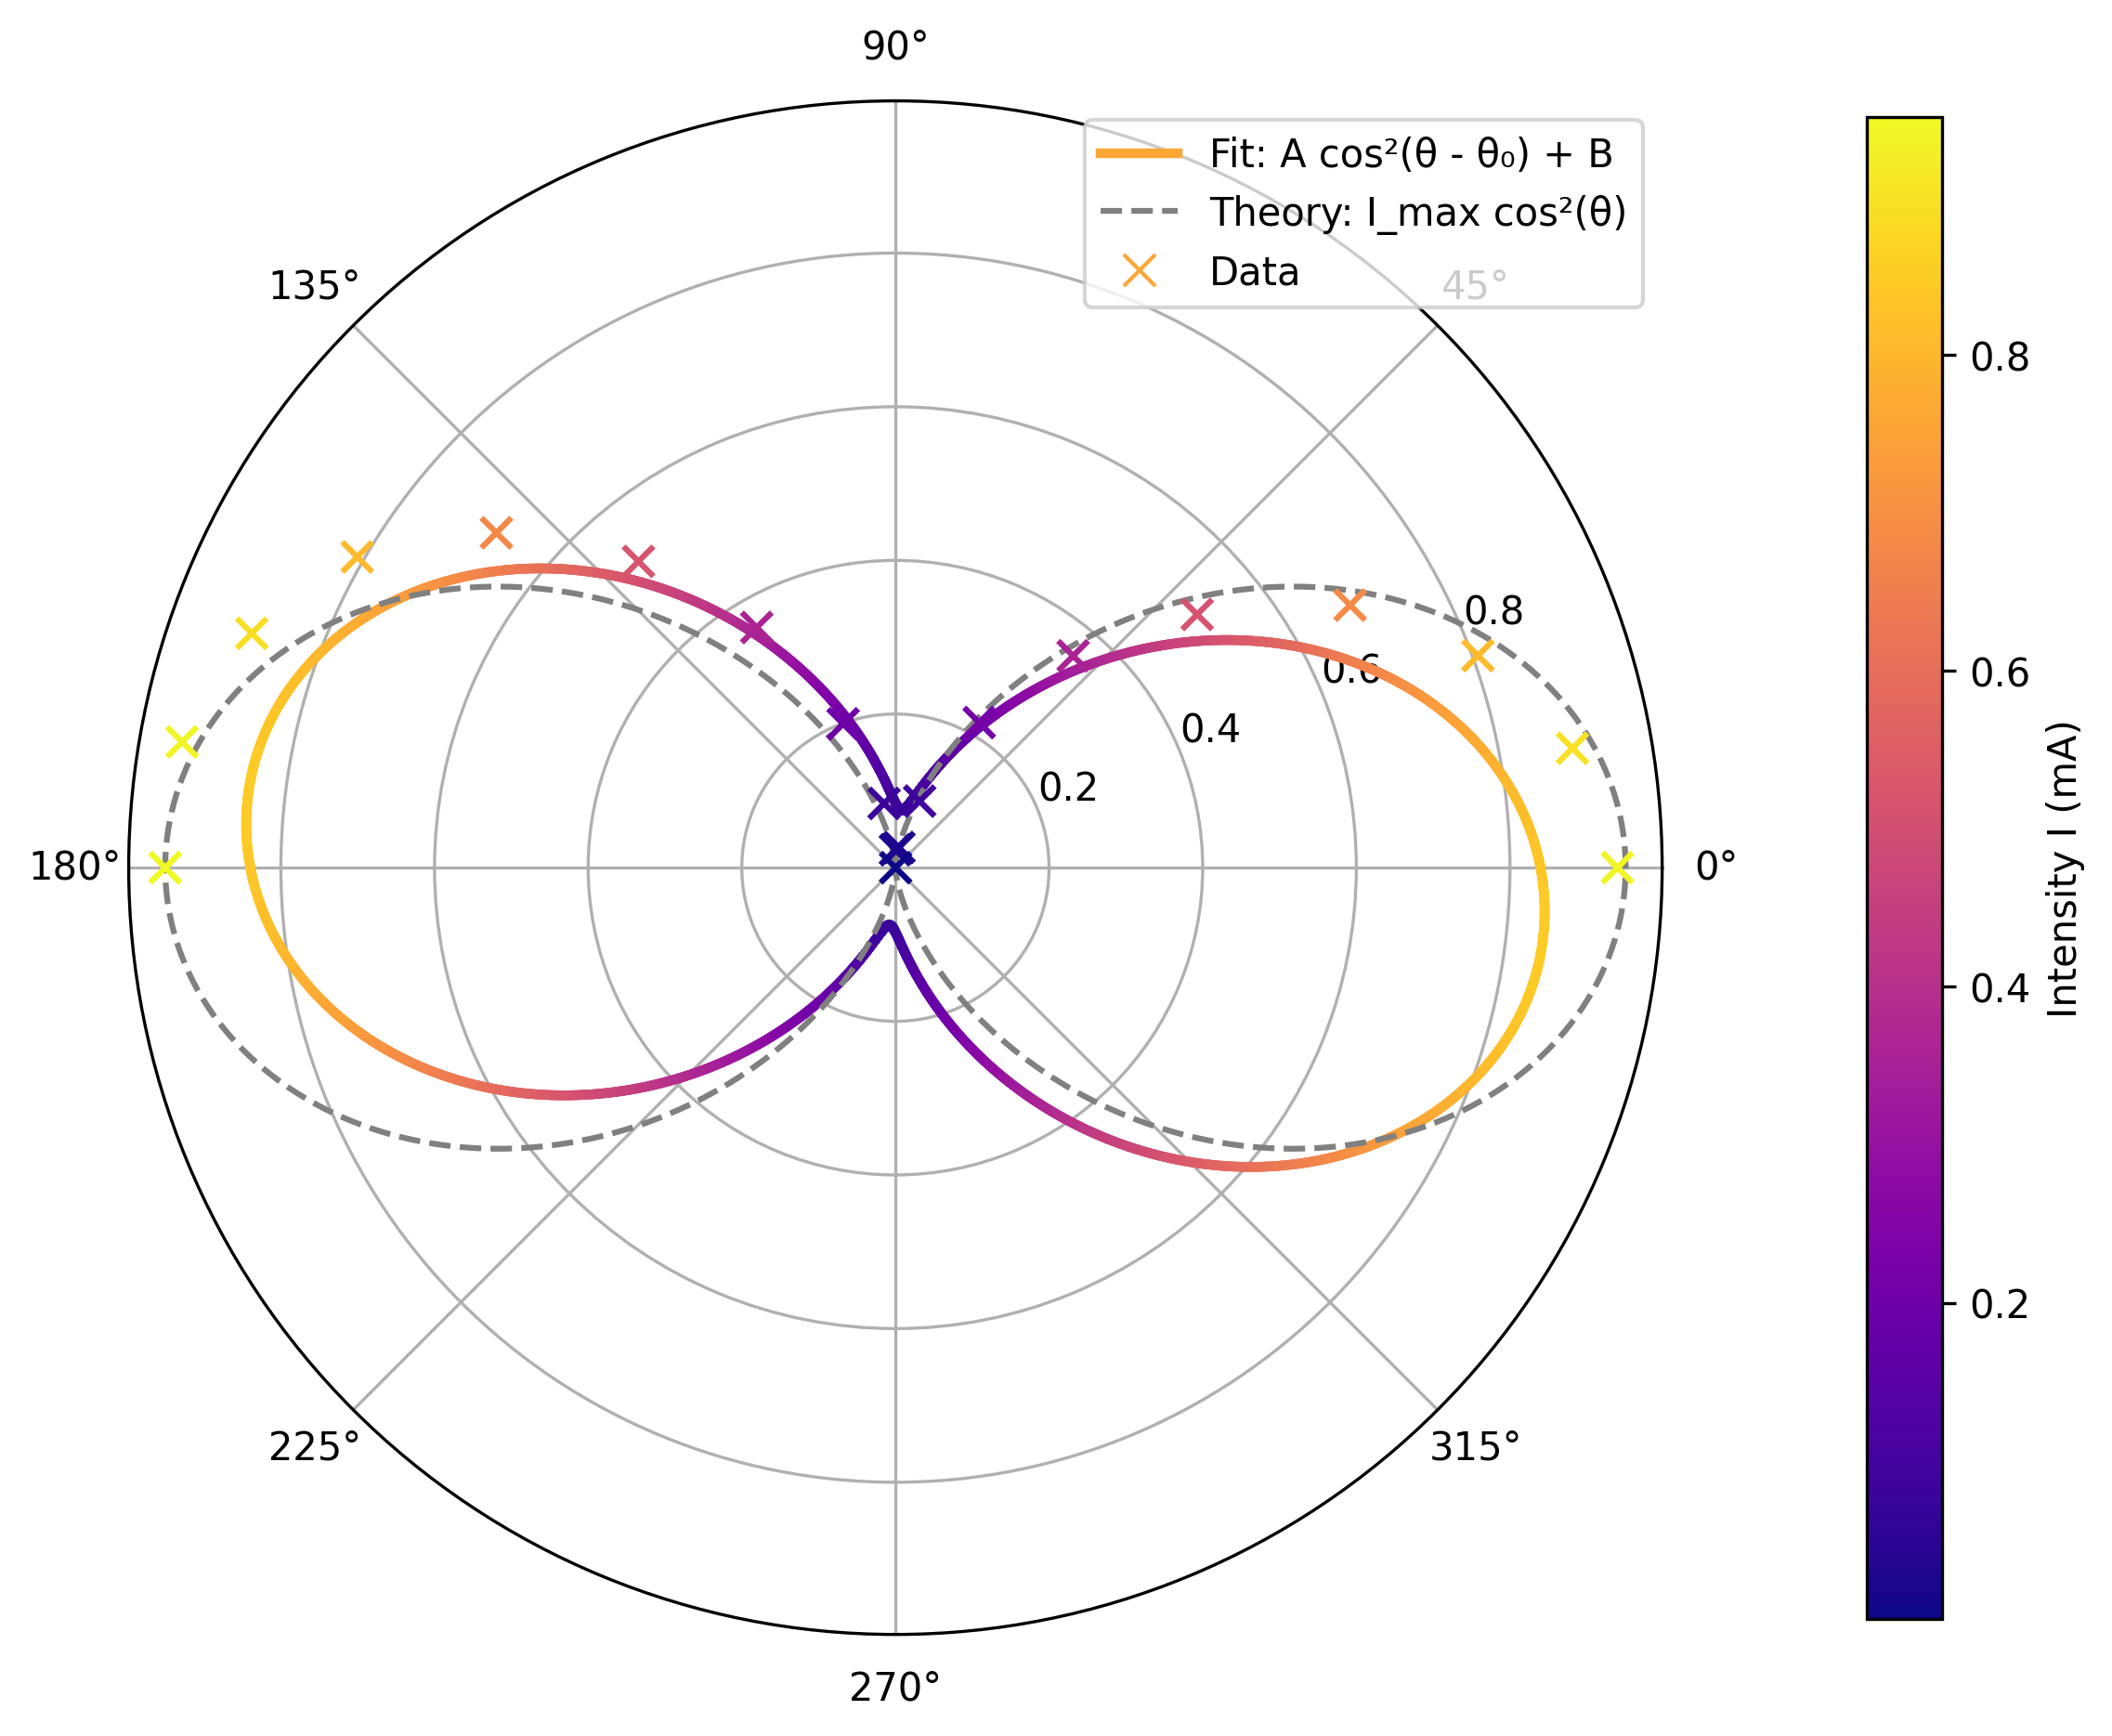
\includegraphics[width=0.5\textwidth]{../Images/Malus_Fit_Polarplot.png}
        \caption{Measured intensity values and the fitted curve with fit $I = A \cos^2(\theta - \theta_0) + B$, $A = 0.7720 mA$, $\theta_0 = -5.95^\circ$, $B = 0.0761 mA$.}
        \label{fig:Malus}
    \end{figure}
    \noindent
    As one can see in fig. \ref{fig:Malus}, for low intensity values, the measured data points fit better to fitted curve, whereas for the angle from $\theta = 
    0^\circ - 90^\circ$ the data points fit good tho the theoretical curve. This indicates, that the measured intensity values are described sufficiently enough
    by Malus's law, but there are some systematic errors in the measurement, which can be caused by the fact that the polarizers are not ideal and do not 
    completely absorb the light that is not transmitted. Another source of error could be, that the room was not completely dark, which could have led to
    additional light being measured by the photocell. Additionally, the angle $\theta$ was not measured with high precision, which could have also contributed
    to the deviations from the theoretical curve.